\section{Introduction}
Many natural systems exhibit fractal properties [\cite{Mandlebrot}]; in fact, scale invariance underlies many self-similar phenomena, from frost crystallization to animal colouration to stock-market pricing. In the realm of optics, the fractal anatomy of systems is widely associated with aggregated dielectric and metal colloids [\cite{Sorensen}], crystals [\cite{Macke}], and tissues [\cite{Schmitt}]. Fractal systems are also observed in nonlinear optics [\cite{Soljacic, Segev}] and fractalized optical properties can even efficiently characterize or enhance the response of materials [\cite{Stockman, Tsai}]. Less well utilized are the features of diffractals, or the diffraction patterns of fractal signals  [\cite{Berry,Horvath,Hou}]. Diffractals feature in methods of encrypting data [\cite{Barrera}] as a versatile approach to double random-phase encoding [\cite{Unnikrishnan}]. However, to differentiate from previous work fractal architecture is exploited to improve transmission robustness.

This chapter explores diffractals for their application in signal processing [\cite{Verma,Verma2}]. Free-space propagation of diffractal-signal architectures provides algorithmic value and spatial multiplexing properties; any arbitrary subsection of a diffractal contains sufficient information to recreate the original sparse signal that is transmitted with a specific fractal architecture. In a manner similar to compressive imaging [\cite{Kelly07, Howland}]\textemdash where sparse signals reveal greater information via the diffraction through structures\textemdash here the fractal structuring within the signal sparseness prevents the loss of information.

Like other applications of fractals in communications applications, the diffractal architecture exhibits trade-offs. Fractal antennas for the radio frequency and microwave regimes are known for being compact and versatile over wide spectral bands but are power intensive [\cite{Radonic,Puente-Baliarda}]; fractal encoding algorithms enable image compression with higher-resolution at the expense of greater algorithmic complexity [\cite{Jacquin}]; this chapter identifies that diffractal architectures prevent the loss of information but require greater signal preprocessing.  This investigation extends the understanding of fractal structures in signal communications and may increase robustness and transmission rates of satellite, wireless, and interplanetary communication systems, {\it i.e.,} networks that support a large number of roaming receivers.

%We analytically, numerically and experimentally show that a fractal structure on a sparse digital signal provides spatial multiplexing and robustness, as well as facile retrieval of the original sparse digital signal. 
The remainder of this chapter is organized as follows.  First, the form of a transmitted fractal signal is formalized, it is shown that the far-field diffraction pattern or diffractal is also a fractal, and the reciprocal nature of fractals is illustrated with the Sierpinski carpet. Second, the robust retrieval of a signal from a diffractal is demonstrated; the original signal is reconstructed even when the majority of the diffractal signal is blocked. Finally, the future applications for diffractal spatial multiplexing in free-space communication systems is discussed. 

\section{Theoretical description}\label{theory} 
\subsection{Spatial multiplexing of the diffractal} 

The fractal transmittance pattern is generated from any base matrix via recursive iterations where the matrix is resized and convolved with itself repeatedly [\cite{Allouche}].  The base matrix $B(x,y)$ adopts a general form,
\begin{equation}
B_i(x,y) = \sum_j\delta(xr^{i-1}-x_j,yr^{i-1}-y_j),
\label{BJ1}
\end{equation}
where the subscript denotes the iteration $i$, $r>1$ is the relative scaling between iterations, and $\delta(x-x_j,y-y_j)$ is the Dirac delta function at $x = x_j$ and $y=y_j$. 
The fractal transmittance function $T(x,y)$ is calculated recursively,
\begin{equation}
T_n(x,y) = T_{n-1}(x,y)*B_{n-1}(x,y),
\label{nTrans}
\end{equation}
where the subscript denotes the order of the fractal or its expression at the $n^{th}$ iteration, $T_0$ is the initial profile of 1's, and $*$ denotes the convolution operator.  

Subsequently, the diffractal is the Fourier transform or the far-field of the transmittance function $\tilde{T}$ [\cite{Horvath}],
\begin{equation}
\tilde{T}_n(k_x,k_y) = \tilde{T}_0(k_x,k_y)\prod_{i=1}^{n}\tilde{B}_i(k_x,k_y)\label{FTn}.
\end{equation}
The Sierpinski carpet is one example of a fractal that is generated by this process and via the iterated substitution of a $3\times 3$ base matrix of ones with removal of the center element:
\begin{equation}
\Bigg\{0\rightarrow \Bigg[\begin{array}{ccc}
0 & 0 & 0 \\
0 & 0 & 0\\
0 & 0 & 0\end{array}\Bigg], 1\rightarrow\Bigg[\begin{array}{ccc}
1 & 1 & 1 \\
1 & 0 & 1\\
1 & 1 & 1\end{array}\Bigg] \Bigg\}.
\label{baseMatrix}
\end{equation}

The second substitution of Eq.~\ref{baseMatrix} represents the mathematical expression for the base matrix $B_0(x,y)$.  In the case of the Sierpinski-carpet base-matrix elements, $r=3$, and $x_j$ and $y_j$ are the perimeter coordinates of a $3\times 3$ 9-unit block centered at the origin, and $(x_j,y_j)\in [(1,1),(1,0),(1,-1),(0,-1),(-1,-1),(-1,0),(-1,1),(0,1)]$. Since each of the Dirac delta functions in $B_0(x,y)$ yields a phase shift in the Fourier domain, {\it i.e.,} $\mathscr{F}\left\{\delta(\alpha x-x_i)\right\} = e^{2\pi i_ck_xx_i}/|\alpha|$, its scaled Fourier Transform at the $i^{th}$ iteration of the Sierpinski carpet [Eq.~\ref{BJ1}] becomes:
%\begin{equation}
%\tilde{T}_n(k_x,k_y) = \tilde{T}_{n-1}(k_x,k_y) r^{n-1}[4\cos(4\pi^2 3^{2(n-1)}k_xk_y)+2\cos(2\pi 3^{n-1}k_x)+2\cos(2\pi 3^{n-1}k_y)]
%\end{equation}
%The amplitude at each iteration is:
\begin{equation}
\tilde{B}_i(k_x,k_y) = (2/r)^{i-1}[\cos(2\pi3^{1-i}k_x)\cos(2\pi3^{1-i}k_y)+\cos(2\pi 3^{1-i}k_x)+\cos(2\pi 3^{1-i}k_y)].\label{BF}
\end{equation}
With each iteration, the spatial frequency components $k_x,k_y$ of the diffractal increase by a factor of 3 and spread the diffractal across a 3-times wider $k_x,k_y$-range, which is evident in Eq. \ref{BF}; the cutoff of $\tilde{T}_n$ scales in proportion with $k_x, k_y \propto r^{n-1}$. 

The Sierpinski carpet, $T$, is calculated recursively [Eq. \ref{nTrans}]: a second-order fractal is generated from the Kronecker tensor product of the base matrix $\Big[\begin{smallmatrix} 1 & 1 & 1 \\ 1 & 0 & 1\\ 1 & 1 & 1\end{smallmatrix}\Big]$ with itself; a third-order fractal is generated from the Kronecker tensor product of a second-order fractal and the same base matrix [see Appendix, \cite{Code1}]. Sierpinski carpets of $n= 1, 3,$ and $5$ are shown in Fig. \ref{AnalRecon}(a) with the corresponding diffractals $\tilde{T}$ [Fig. \ref{AnalRecon}(b)]. 

%\lstset{language = Matlab}
%\begin{lstlisting}
%function carpetHolo = Sierpinski(fracOrder);
%	carpetBase = ones(3); % Initialize matrix
%	carpetBase(2,2) = 0;
%	% Zero middle element
%	if fracOrder==0;
%		% For zero order case
%		carpetHolo = carpetBase;
%	else
%		% For higher order cases
%		carpetHolo= kron(carpetBase,carpetBase);
%		% For loop iterates the Kronecker tensor product
%		for i = 1:fracOrder-1
%			carpetHolo = kron(carpetHolo,carpetBase);
%		end
%	end
%end
%\end{lstlisting}

As the fractal order increases, $\tilde{T}$ exhibits smaller self-similar features at higher $k_x,k_y$;  the diffractal also exhibits a fractal architecture, as observed in other literature [\cite{Berry,Horvath}].  Moreover, when $n$ is large, an arbitrary subsection of $\tilde{T}$ closely resembles the whole, and the self-similarity is already apparent with $n= 5$ [Fig. \ref{AnalRecon}(c-d)]. The iterated, self-similar, wide-spatial-frequency features contained in the diffractal $\tilde{T}_n$ [Eq. \ref{FTn}] enable robust reconstruction of itself, which is described in the next subsection.

\begin{figure}[t!]
 \includegraphics[width=\textwidth]{AnalyticalHolgramReconstruction.pdf}
\caption{(a) Signal patterns, or fractalized signals (FS) of orders $n = 1$, $3$, and $5$. (b) Corresponding Fourier transforms of signals on logarithm scale, or diffractal signals (DS). (c) Reconstructed Fourier-transforms (RFS) from the 1\% black-outlined subset, the blocked diffractal signal (BDS). (d) Enlargement of a portion of the $n=5$ diffractal, which illustrates similar patterns at different length scales.}
\label{AnalRecon}
\end{figure}

\subsection{Robust reconstruction of a blocked diffractal signal} 

The sparse matrix $B_0$ and transmitted signal $T$ are referred to as the original and fractalized signal, OS and FS, respectively; the diffractal signal DS is $\tilde{T}$, or, the Fourier transform of FS; BDS refers to an off-axis subsection of DS that is filtered; a reconstructed fractalized signal RFS refers to the inverse-Fourier transform of BDS; a regenerated version of the original signal ROS interpolates RFS in order to obtain OS.  

In Fig.~\ref{AnalRecon}(b), a subsection or BDS is outlined with a black square, which represents 1\% of DS. The corresponding RFS from BDS are shown in Fig. \ref{AnalRecon}(c). For $n$ = 1, 3, RFS is ostensibly blank because BDS carries negligible power.  In contrast, when $n=$ 5, RFS carries features that resemble FS. The capacity to reproduce FS with 1\% of the off-axis area from DS is referred to as ${\it robust}$ reconstruction.  

Robust reconstruction\textemdash where RFS resembles FS\textemdash is possible even when the size of BDS is significantly reduced [\cite{Verma}].  A corresponding increase in the FS fractal order $n$ will yield RFS that resembles FS when BDS is arbitrarily small. With the example of the Sierpinski carpet, Fig. \ref{AnalRecon}(a)--\ref{AnalRecon}(c), if the size of BDS is reduced to 1\% of OS, then a comparable RFS is produced by increasing the fractal order of FS from $n=1$ to $n = 5$. 

Robust reconstruction is defined as the capacity to regenerate OS from RFS from a simple threshold function [see Appendix, \cite{Code2}]. The threshold function of the Sierpinski carpet divides RFS into a $3\times 3$ array (identical size as OS) and measures the intensity in each of the 9 elements. Above a certain threshold value, the element is assigned a value of 1, and otherwise assigned a value of 0. The $3\times 3$ array that is processed with the threshold function, ROS, is theoretically identical to OS when OS is transmitted with the diffractal architecture. 

%\begin{lstlisting}
%function recon = reconFun(Threshold,carpetBaseLength,carpetHolo)
%	% Ratio of length of hologram
%	normLength = length(carpetHolo)/carpetBaseLength; 
%	
%	% Convert to array of cells
%	cellHolo = mat2cell(carpetHolo,repmat(normLength,1,...
%	carpetBaseLength),repmat(normLength,1,carpetBaseLength));
%	
%	% Calculate mean, determine if above threshold value, and plot
%	pcolor(double(cell2mat(cellfun(@mean2, cellHolo))>Threshold));
%end
%\end{lstlisting}

The comparison between RFS and FS in peak signal-to-noise ratio (PSNR) for various fractal orders as a function of the fractional BDS size is shown in Fig.~\ref{PSNR}. The error bars represent the standard deviation from the mean value of 200 random locations of BDS. Since the size of RFS is reduced from FS, RFS is resized with nearest-neighbour interpolation. 2 observations from Fig.~\ref{PSNR} are provided: first, when BDS is greater than 0.01\% of the fractional size of FS, larger fractal orders produce higher PSNR; second, as the fractional area of BDS increases the location of BDS becomes irrelevant since the standard deviation around the mean diminishes. For fractional BDS sizes smaller than 0.01\% lower fractal orders yield a higher PSNR since the minimum size matrix needed to completely recreate FS is larger for higher fractal orders. For example the minimum size matrix needed to recreate FS of order 1 is $3\times 3$, for FS of order 2 it is $9\times 9$, etc. 

\begin{figure}[t!]
\begin{centering}
 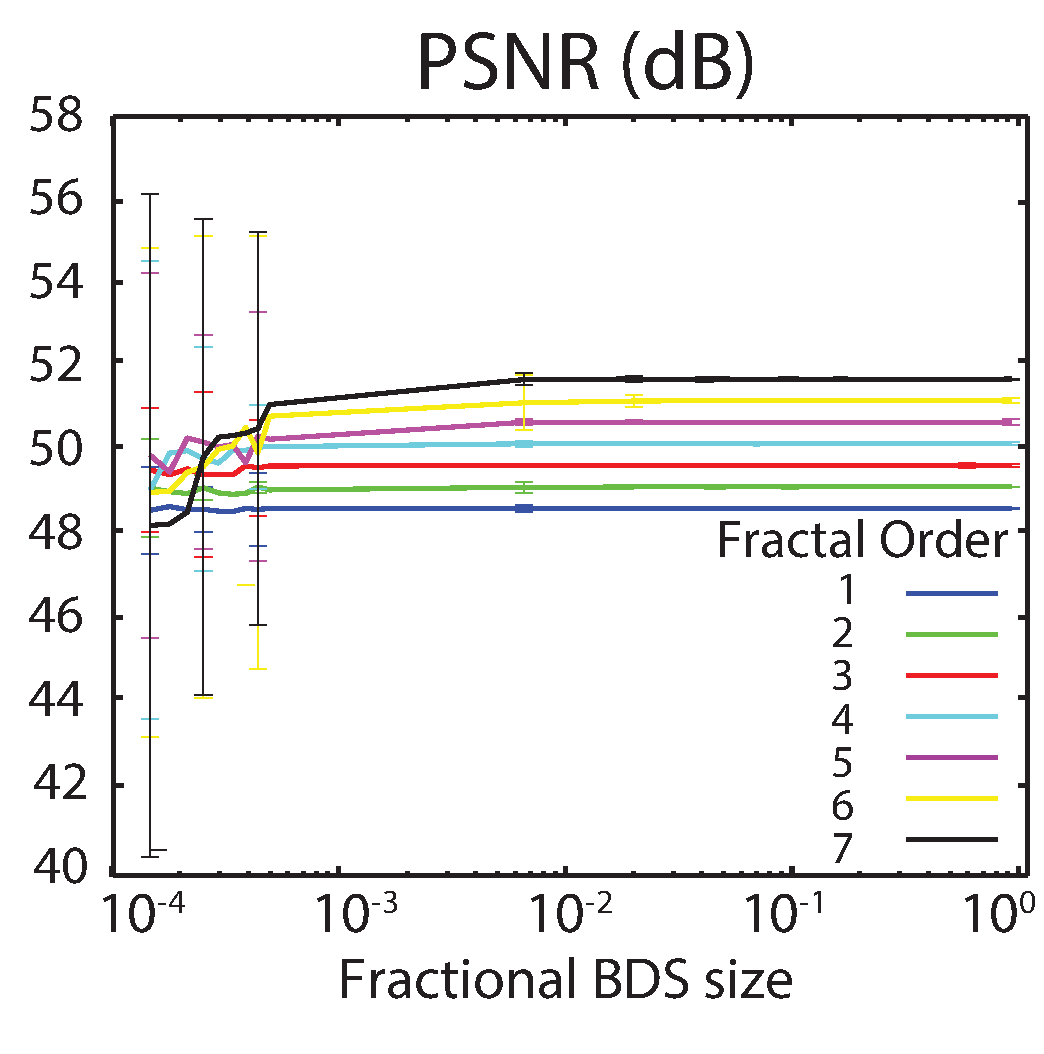
\includegraphics[width=0.7\textwidth]{psnr_good_eb2.pdf}
\caption{The peak signal-to-noise ratio (PSNR) of RFS to FS for various fractal orders as a function of the fractional BDS size.}
\label{PSNR}
\end{centering}
\end{figure}

ROS is generally identical to OS when BDS is above 0.01\% and the fractal order is greater than 3, regardless of BDS location. A partial explanation for the robust reconstruction is that increasing-order FS carry arbitrarily-high $k_x,k_y$ and enable arbitrarily-{\it small} BDS to carry the information of FS or OS.  If OS is strictly limited to binary or Dirac-delta functions, then FS has no $k_x,k_y$ cut-off and as $n$ approaches infinity, fractalized features appear in FS without a $k_x,k_y$ cut-off.  In fact, the amplitude of the additional $k_x,k_y$ gained from each iteration scales inversely with $r^{n-1}$, which provides a detection limit only in practice; in theory, each iteration generates high-$k_x,k_y$ copies of OS [Eq.~\ref{baseMatrix}] that are spatially distributed from the origin.  

Yet it is worth noting that the robust reconstruction is achieved because the diffractal architecture also couples $k_x$ and $k_y$ in iterated products [Eq.~\ref{FTn}].  As a result, RFS will resemble FS when either the BDS size {\it or location} changes.  In a manner similar to spatial filtering, RFS will produce outlines of FS if $n$ is not sufficiently large; however, unlike a high-pass spatial filter of a multi-scale random high-$k_x,k_y$ pattern [\cite{Kelly07}], a change in the location or the size of BDS will not distort the outline of RFS.  Subsequently, the diffractal architecture provides superior performance over other algorithms that regenerate sparse data, OS [\cite{Kelly07, Howland}].   


%\begin{equation}
%H = \frac{1}{2m}(p_x^2 + p_y^2) + \frac{1}{2} M{\Omega}^2
%     (x^2 + y^2) + \omega (x p_y - y p_x).
%\end{equation}

\section{Experimental results} \label{experiment}
\indent The features of diffractals are experimentally demonstrated with a 4-$f$ optical arrangement where the 2-dimensional Fourier transform of a collimated fractal image, DS, lies in the focal plane of an imaging lens \cite{Goodman}.  The experimental setup that produces, filters and reconstructs FS is shown in Fig. \ref{ExpSetup}(a) and experimentally reconstructed images, RFS, are shown in Fig. \ref{ExpSetup}(b). An aperture of area approximately $0.8mm^2$ blocks the majority of DS. The placement of the aperture is shifted roughly $4mm$ horizontally and $5mm$ vertically from the central point, in the focal plane of the lens. The SLM image has a resolution of 800$\times$600 pixels (16mm$\times$12mm).  

\begin{figure}[t!]
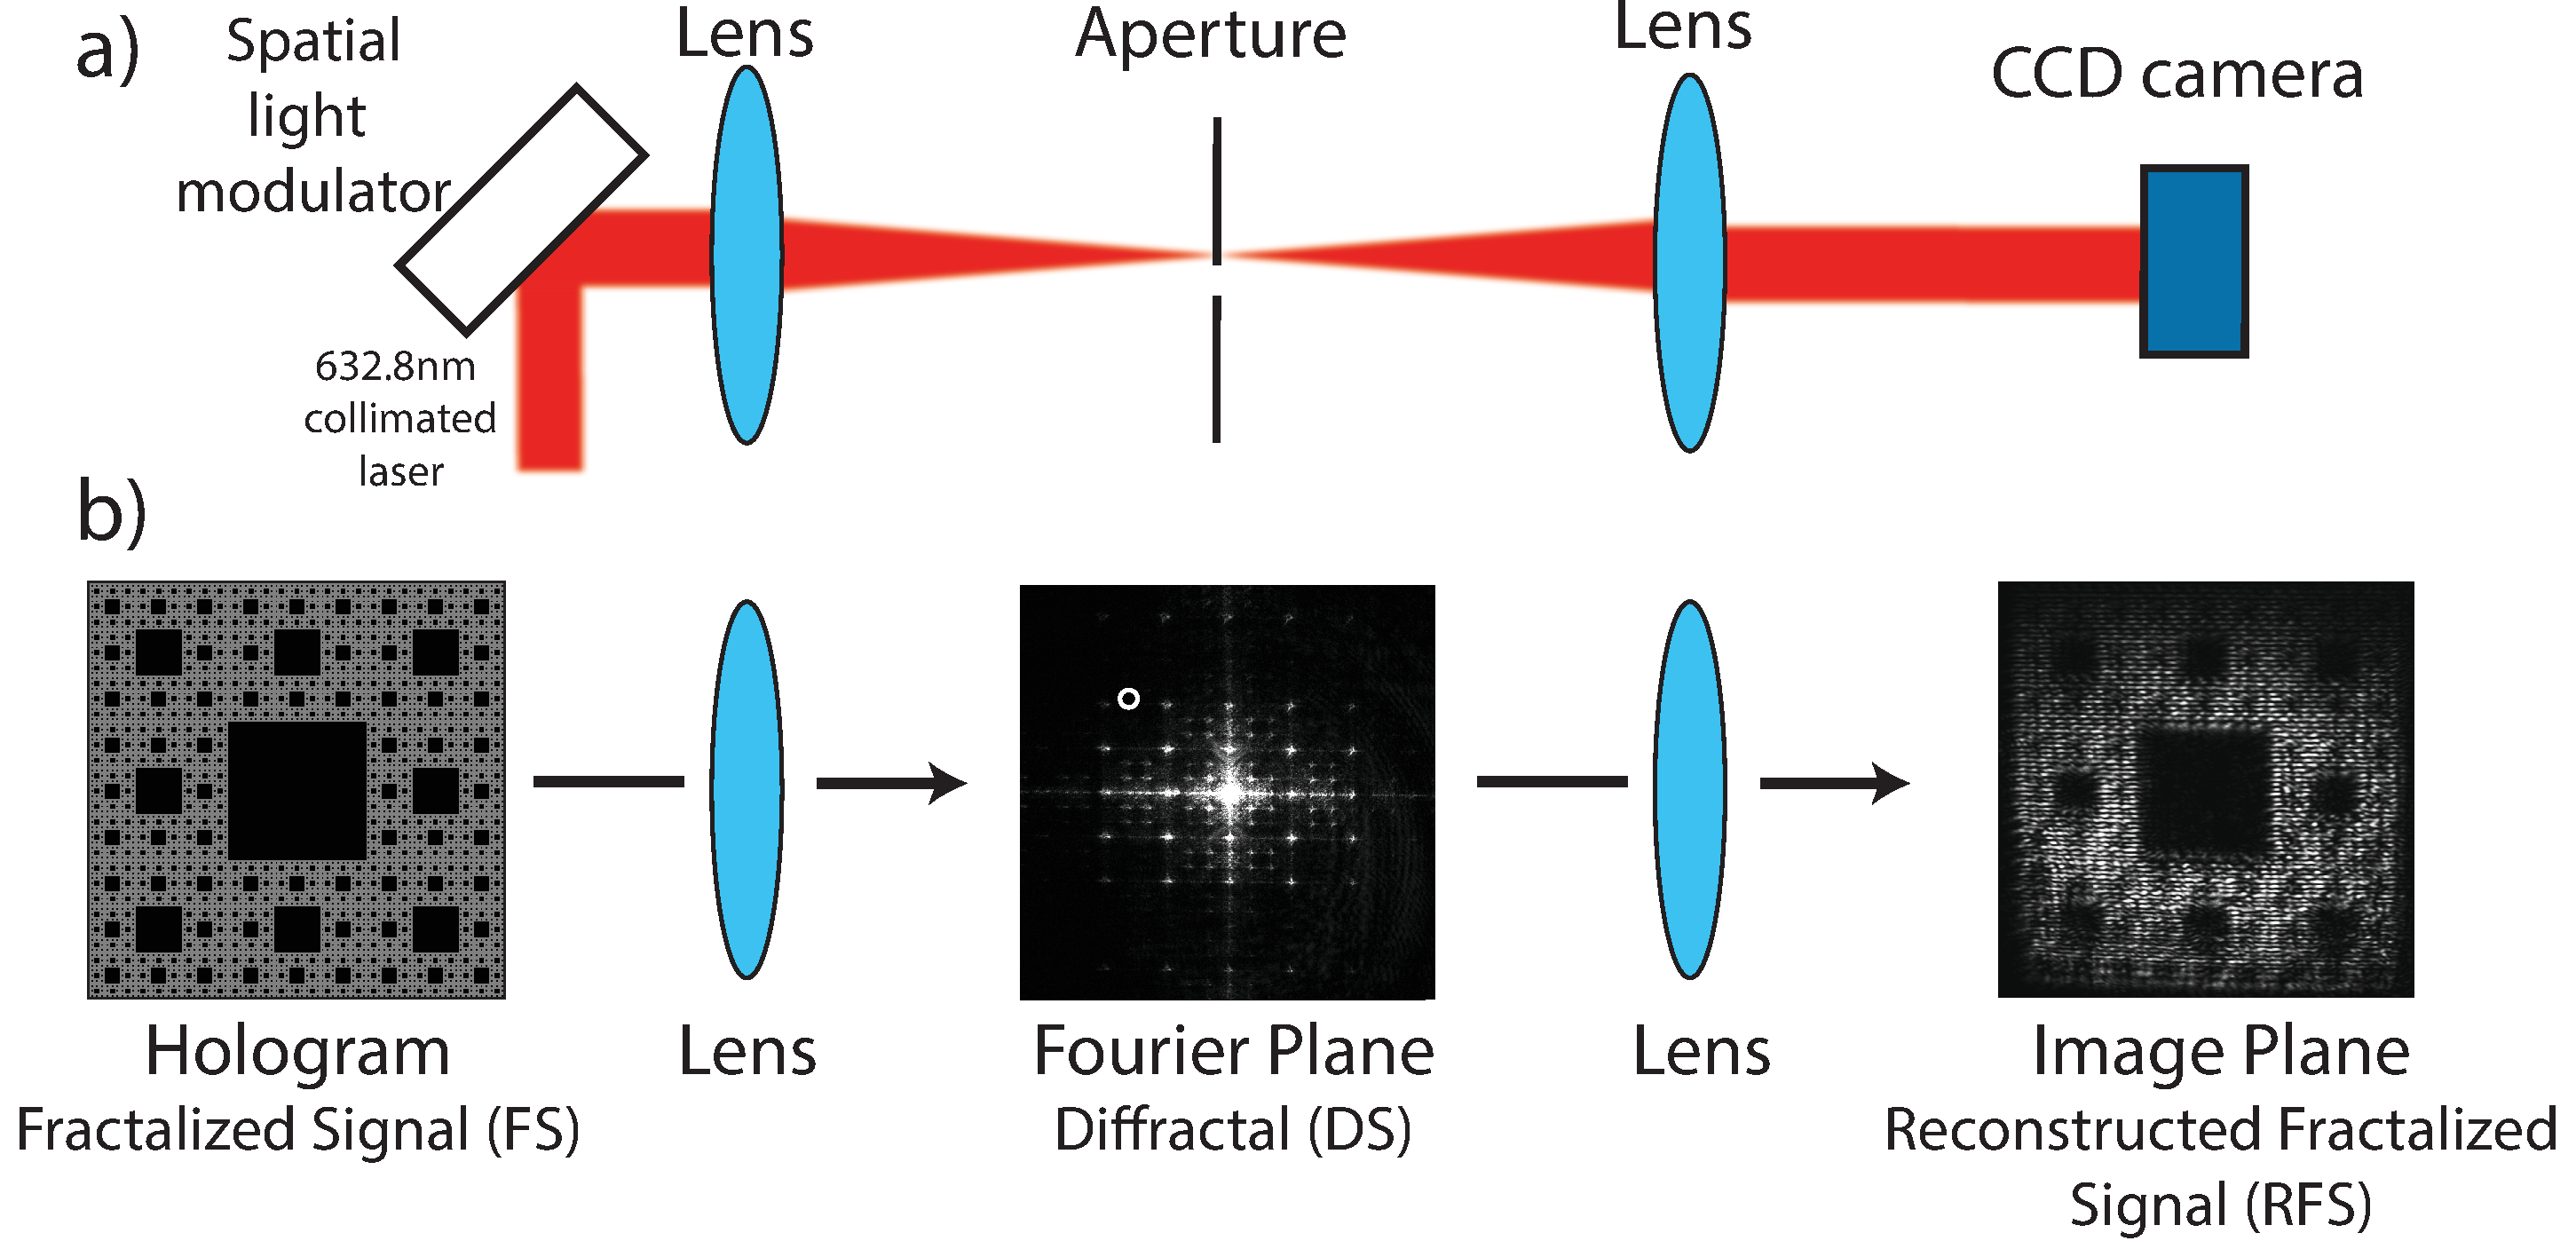
\includegraphics[width=\textwidth]{ExpMethod.pdf}
\caption{(a) Light from a $\lambda = $ 632.8-$nm$ wavelength laser is spatially filtered, expanded, and collimated and illuminates the full area of a 800x600 pixel spatial light modulator (SLM). The 4-$f$ system is composed of 2 5-$cm$ lenses placed after the SLM. The first lens Fourier transforms the fractal signal (FS) at the focal plane. An aperture is placed off-center at the focal plane and only transmits a portion of the diffractal (BDS). The second lens reconstructs the SLM image with the light that is transmitted through the aperture. (b) The Sierpinski carpet hologram of order $n$= 5, CCD image in the focal plane of the hologram after the lens, and the reconstructed image. A circle denotes the area utilized to reconstruct the image.}
\label{ExpSetup}
\end{figure}

When high order diffractal architectures are employed ($n>$4), a phenomenon is observed that is shown numerically: the placement of the aperture in DS is irrelevant in order to reconstruct the original image. When the aperture is moved laterally in the focal plane, RFS maintains strong resemblance to FS. In fact, only the intensity of RFS diminishes as the aperture translates further from the DS center; the outline remains fixed as the aperture moves.  For smaller fractal orders, RFS resembles FS only when the aperture is placed within $0.8mm$ of the center, where the spatial frequency components are concentrated. The signal-to-noise of the experiment and CCD camera sensitivity limit effective reconstruction, while the highest order $n$ is of FS is limited by the number of SLM pixels.  

\section{Discussion of applications}\label{disc}
A distinction is made that diffractals are specific fractal structures. Not all fractals enable robust signal communications and the recursive transformation employed to generate FS and DS in Eq.~\ref{BJ1} and~\ref{BF} differ fundamentally. For example, both of the Fourier Transform pairs FS and DS are fractals and carry iterated, self-similar features, but if the roles were reversed in the transmission system, the reconstruction will instead depend severely on the size and location of BDS. In fact, if in the example of the Sierpinski carpet, the center subsection becomes BDS, then the ROS will not resemble the OS, regardless of fractal order.  The diffractal is unique from general fractals and self-similar scale-invariance alone is an insufficient precondition for our system of robust reconstruction and spatial multiplexing. 

It may seem contradictory that higher-order fractals lead to more robust signal transmission since the finer structure of a higher-order fractal is itself harder to reconstruct. There are two perspectives of diffractals that explain the robust reconstruction. First, the self-similar structures of higher-order fractals have a greater spatial frequency range and finer detail, and subsequently smaller BDS carry sufficient information to reconstruct OS. Second, the higher-order diffractals carry higher spatial-frequency components where the $k_x$ and $k_y$ components are coupled, and subsequently the location of the subsection in DS is unimportant. In these experiments BDS of arbitrary size and location carry sufficient information to reconstruct OS but in practice, there exists clear limitations for the robust reconstruction even in the limit of infinite-order FS.  

Note: it may also seem contradictory that an infinitesimally-sized BDS with infinitesimal power can carry information-- this is not actually true: there is a minimal size for BDS fixed by the pixelation of the SLM.
There exists a trade-off with the diffractal architecture between robust reconstruction and high bit rate; a greater bit-rate is achieved with a larger base matrix, which can limit the maximum fractal order that is transmitted.  For example, with the $3\times 3$ or 9-element OS, there are 512 possible spatial bits, three of which are illustrated in Fig. \ref{Multiplex}(a-c).  A $4\times 4$ base matrix requires $(\frac{4}{3})^{2n}$ more pixels than a $3\times 3$ to achieve the same fractal order, $n$. With a limited SLM pixel resolution, there is a choice between the generation of higher-order fractals and the utility of higher spatial bits.   

If the trade-off between bit-rate and robust reconstruction are mitigated, then the diffractal architecture could support a large number of roaming receivers with only one transmitter, such as wireless or satellite networks shown in Fig. \ref{Multiplex}(d). The self-similar properties of the diffractal architecture and their corresponding far-field pattern provide a method to reach a large number of receivers, possibly moving, without signal degradation.  The processing times required in the calculation of FS from OS are not trivial and scale with $r^{2n}$. Furthermore, the refresh rates of a spatial light modulator or similar adaptive-optics device present constraints on the maximum achieved bit rate, which requires further consideration.  

\begin{figure}[t!]
\includegraphics[width=\textwidth]{Multiplexing2.pdf}
\caption[]{Three examples of 512 9-bit spatial patterns, associated with base matrices 
(a) $\Big[\begin{smallmatrix} 1 & 0 & 1\\ 1 & 1 & 1\\ 1 & 0 & 1 \end{smallmatrix}\Big]$, (b) $\Big[\begin{smallmatrix} 1 & 1 & 0 \\ 0 & 1 & 1\\ 0 & 1 & 1\end{smallmatrix}\Big]$, and (c) $\Big[\begin{smallmatrix} 1 & 0 & 0 \\ 1 & 1 & 0\\ 1 & 1 & 1\end{smallmatrix}\Big]$. The fractal signals FS are shown with their corresponding experimentally-reconstructed fractal signals RFS from the experimental setup in Fig. \ref{ExpSetup}(a).  The lower-right inset shows the reconstructed original signal ROS. (d) Example application: transmitted fractal signal FS is received at a far-field distance as a diffractal signal DS, where a roaming set of receivers, with only a diffractal subsection BDS, reconstructs the original signal OS.}
\label{Multiplex}
\end{figure}
This can be applied to more complex shapes and structures, for example, an $16\times 16$ pixel smiley face shown in Fig.~\ref{face}. The Fourier transform of the smiley face is taken; part of the Fourier transform is blocked; and a reconstruction of the image is attempted via the inverse Fourier transform. The same experimental procedure as shown in Fig.~\ref{ExpSetup} is utilized. As can be seen from Fig.~\ref{face} when just the image is sent through the experimental setup the image reconstructed is not recognizable at all. However when the image is fractalized even just one order the image becomes recognizable. Unfortunately due to the limitations of pixels on the SLM no higher orders can be achieved.\\
\begin{figure}[h!]
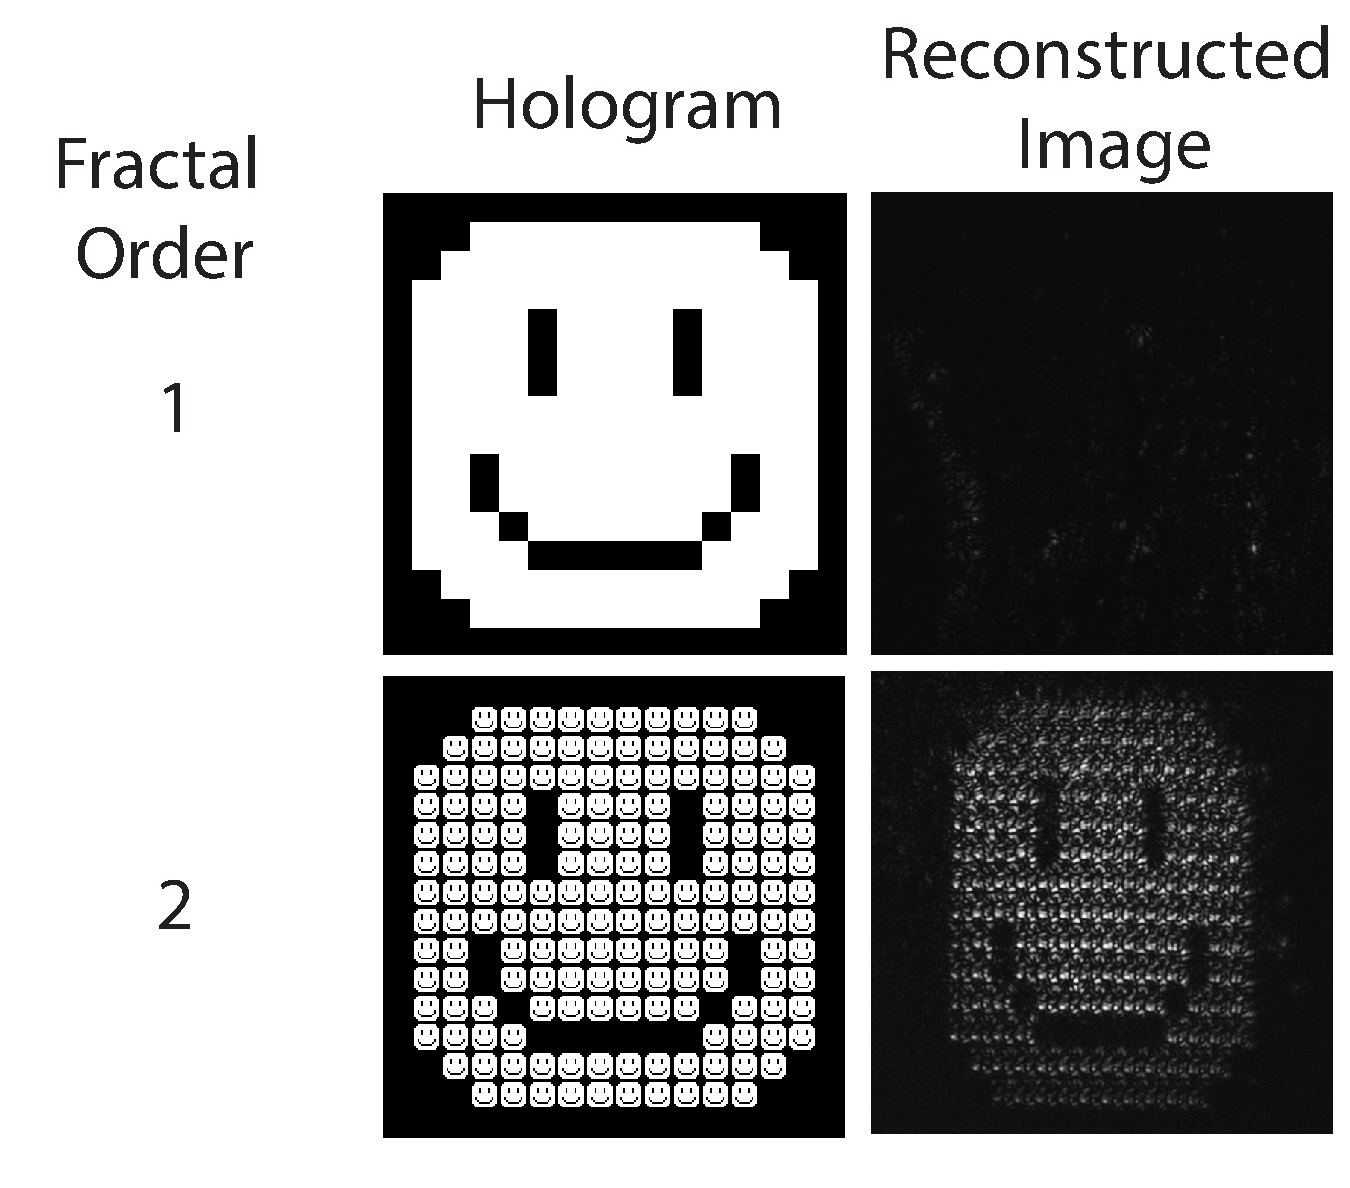
\includegraphics[width=\textwidth]{imgRecon.pdf}
\caption[]{As an example of a more complicated image, a smiley face is fractalized, the Fourier transform is taken, 99\% of the signal is blocked at the focal plane, and the image is reconstructed. This is compared to the original signal that is not fractalized.}
\label{face}
\end{figure}

Fractal structures have been utilized in signal communications and data compression for decades. Fractal antennas for the radio frequency and microwave regimes are known for being compact and versatile over wide spectral bands [\cite{Radonic,Puente-Baliarda}]. Fractal encoding algorithms enable image compressing with higher-resolution compression at the expense of greater algorithmic complexity [\cite{Jacquin}]. The trade-off for higher resolution fractal-compressed images is higher processing times, which presents a limitation of their presence in data communications. Recently, however, there has been a resurgence of interest in fractal architecture due to their robust properties in optical transmission.

\section{Conclusion}
This chapter has shown that the diffractal architecture provides the beneficial features of spatial multiplexing and robust reconstruction. Demonstrations have been shown with the Sierpinski carpet, a familiar fractal, although the results could have been demonstrated with 511 other patterns similarly imprinted with the diffractal architecture. Data that is transmitted with the diffractal architecture is highly robust to intermediate-obstacle signal blocks and diffractal subsections of arbitrary size and location carry sufficient information to regenerate the original signal without distorting outlines of its pattern.  This research illuminates potential applications in data transmission systems when one transmitter sends data to a large number of moving receivers or through noisy media.

\section{Experimental difficulties and future work}
A SLM works well for experimentation because of its facile reconfigurability, however the resolution is limited to 800$\times$ 600 pixels, that limits the complexity of the data image sent in the process. Ways to overcome this could be to use photolithography to create transmission structures with a larger pattern on a glass film, however the structure would lose the reconfigurability that the SLM possesses. Transmission could even be created by printing the transmission structure pattern on transparency sheets, which would be a cheap alternative method to achieve similar results with a lower resolution.